\documentclass{article}

\usepackage[british]{babel}
\usepackage[T1]{fontenc}

\usepackage{hyperref}
\usepackage{biblatex}
\addbibresource{nea.bib}

\usepackage{adjustbox}
\usepackage{tikz}

\usepackage{minted}

\usetikzlibrary{shapes.misc}

\tikzstyle{flowchartbox} = [text centered, draw, minimum width=3cm, minimum height=1cm]
\tikzstyle{terminal} = [flowchartbox, rectangle, rounded rectangle]
\tikzstyle{process} = [flowchartbox, rectangle]
\tikzstyle{flowchartarrow} = [->,thick,>=stealth]

\author{Nils André-Chang}
\title{NEA: OCR Exam Reference Language as a Language, an implementation}

\begin{document}

{\huge THIS COPY OF THE DOCUMENT IS A DRAFT AND IS NOT MEANT TO BE MARKED}

\maketitle

\tableofcontents

In this document, the author refers to themselves as `we' however, there is
only a singular author, and the use of this pronoun is not meant as an
indication of there being multiple authors.

An implementation of the OCR Exam Reference Language as defined by
\textcite{j277, h446}.

\section{Analysis}

\subsection{The problem and its computational solution}

Every year in the UK, thousands of students take computer science as a subject
for their secondary school education; in the summer of 2019, 11124 took it for
A Levels, 3098 for AS Levels, and 80027 for GCSEs
\cite{jcqalevel19, jcqgcse19}.

In order to assess the ability of the students in the subject, two methods are
used: examination and non exam assessment (NEA) in the form a programming
project. To assess students during exams, exam boards produce questions that
use and ask the student to use a pseudocode that is language agnostic and has
been predefined in the specification of the exam board. This is done for
clarity and consistency among other reasons \cite{h446, j276, j277}.

Such an exam board is OCR: in \textcite{h446, j276, j277} a pseudocode is
defined, in \textcite{j277}, it was renamed to ``OCR Exam Reference Language''.

The problem with having a relatively strictly defined language is that although
it is called a ``pseudocode" (at least in older specifications) and it is
mentioned that ``Learners [...] may provide answers in any style of pseudocode
they choose providing its meaning could be reasonably inferred by a competent
programmer.'', it is often that students lose mark due to the style of
pseudocode they chose not being understood by the examiner for various reasons.
As a result of this, it is preferable for students to write their answers in a
style that is as close as possible to the ``pseudocode'' defined by the exam
board to avoid losing marks.

From here on out, what has been described as the `pseudocode' will now be
referred to as a language this is because, firstly, we believe that as an
inherent result of the language used in OCR exams being defined within the
specification, it is no longer a pseudocode but in fact a programming language.
Secondly, in the newest computer science specification, \textcite{j277}, what
was previously described as a pseudocode, is now known as the ``OCR Exam
Reference Language'' (We suspect it is because of the realisation of point 1 by
OCR although there is no evidence to this).

Unfortunately, learning a language is complicated and one of the best ways to
learn one is to practice with it. However because the language is only defined
in the specifications of exam boards, there is no way to practice using it, as
there is no way to execute any code written using the syntax of this language.

Another problem that stems from the use of this language as described is that
there is no way to check in a reliable way if code written using it is correct.
Whether that is when a student is practicing for exams or when writing exam
papers themselves. In the June 2018 A Level Paper 2, there was a mistake in the
exam paper students had to take, demonstrating that even the most proficient
can make mistakes \cite{ocrpec18}.

% TODO how is computation better than other solutions.

We believe that a solution for the problems described would be to implement the
language, as described in the specifications and as used in exams, such that
users can run code that was written using the language. The problem described
lends itself particularly well to a computational solution and in fact is the
only possible solution as computers are the only way to execute and trace
software in a reliable way: although humans can trace the execution of a
program it is a very error prone operation. Additionally, the purpose of this
language is to check a human's work which inherently means it will have to use
another method than one that is carried out by a human: a computer.

If there was the possibility to run the code, it will allow students to use the
language when going through the GCSE and A Level courses which will allow them
to learn the language well and then be able to use it confidently within the
exam. This will improve their ability and allow them to score higher in exams.
Being able to execute code written in this language will also allow to check
answers when practising giving students practical ways to verify what they are
doing; this is especially important at GCSE where students are not necessarily
confident enough to be able to tell for themselves if something is correct and
why it is correct. Lastly being able to execute code written in this language
will also allow to check code that was written using it for example for the
purpose of exam papers removing the possibility of mistakes creeping up like
they did in the June 2018 A Level paper.

Another advantage of having a working implementation of this language is that
students will no longer need to learn two languages: a programming language and
the OCR Exam Reference Language. They will be able to only learn the OCR Exam
Reference Language because they will now be able to use it as a proper
programming language and write programs using it.

Although this project will focus on the OCR Exam Reference Language, this
section in particular applies to other exam boards. The problems described here
are not specific to OCR.

% TODO reference to the sections

From here on out, the result of this project will be referred to as an
implementation of the language, this is because the specifics of the
implementation have not been well defined yet and will be in the features and
the design section.

\subsection{Stakeholders}

One of the main stakeholders for the project are the users. There will be
many different types of users but a majority of them will fall under one of
four different categories: exam board and resource producers, students, and
teachers.

The exam boards and resource producers will make a similar use of the
implementation of the language: they will use it to create resources, one
mainly in the form of exams and the other in a wide variety of forms: exam
style questions, practice activities and other learning resources.
\Textcite{pattis88} found that 80\% of textbooks implemented binary search
\textbf{in}correctly and the 2018 A Level OCR paper contained an error in the
code they presented students suggesting errors in code presented to students
can arise easily and solutions need to be found. We believe that using an
implementation of the language is one such solution and will reduce the
occurrence of this mistake. Exam boards and resource producers will be able to
use the implementation to verify through testing that correct code is produced
in mark schemes, exam questions, and other resources. Exam boards and resource
producers have a very strong interest in creating high quality material with
the least amount of mistakes in them in order to maintain a reputation which
leads to their product being used and purchased (whether that be exams or
preparation material). Furthermore, exam boards have previously been fined for
mistakes in exams \cite{ofqual20180702} and resource producers could also be
sued if the content they produce lead to students failing their qualifications.
For this reason, using this an implementation of the language will not only
improve the accuracy or resources it will also reduce costs (in forms of fines)
for exam boards and resource producers.

Another group of users of the language will be students who are studying
computer science in secondary school. They will be able to use the
implementation to check their answers to questions as well as to write programs
as part of their learning. We believe that this will help boost their grades in
2 ways: firstly, being able to check their answers reliably will allow them to
answer and check their responses in less time leading to them doing more
effective practice and will allow them learn the fundamentals of programming
rapidly and be more confident with their learning as they can prove that what
they have learned works; secondly, having to learn only a single language will
reduce the amount of learning necessary which will allow them to have a more
focused learning and know the content they need to know better.

Lastly, the language can be used to check the answers of students, by running
the programs using the interpreter and verifying the output. This is a task
performed mainly by exam boards and teachers. Exam boards will be able to use
the language to mark some of the work produced by students in exams reducing
the likelihood of mistakes done by markers and being more lenient as long as
the student wrote a valid program. Teachers will also be able to use it to plan
their lessons and demo some of the programs to their students, making the
lessons more engaging.

In addition to users, stakeholders may include companies and individual who
extend the language for profit or not. This includes developers of editors and
other integrated development environments. For example a company could create
an online platform for students to try the language out or save their code.

\subsection{Existing solutions}

Currently what is done is that when people write code in the OCR Exam Reference
Language they can only check it manually, this can be considered to be a
solution however it is error prone and doesn't provide much, in particular to
students who are not proficient in the language.

There are however other software that have been written in the past that are
much more similar to what this project aims to offer.

\subsubsection{Existing programming languages}

Programming languages are not a new concept, they have been a major subfield of
computer science since its inception and are still one of the major ongoing
areas of research. As part of the project, we will be developing an
interpreter. Interpreters have been written thousands if not millions of times
before, virtually every programming language has an interpreter, as such there
is a lot of documentation and resources explaining how to write interpreters
and programming languages and it is for the most part a solved problem.

In order to develop this programming language we will use \textcite{eopl}, a
textbook that is used in many programming languages university courses around
the world, to guide us.

We will also inspire ourselves from other languages. In particular
\citetitle{python}, and \citetitle{rust} in order to derive the intended
behaviour of the OCR Reference Language when it has not been defined well
enough in the specification. What we mean by that is when we are not sure how
our program should behave we will try to match the behaviour that would be
displayed by rust or python.

The reason for these 2 choices is that python is one of the most popular
programming languages as of the time of this writing and is the one used by
most schools to teach their secondary school students, additionally the OCR
Reference Language is very similar to python and as such we believe that
drawing its behaviour from python is most likely to be what is intended.
However sometimes we will match the behaviour of rust as it is the language we
will use for the implementation and thus it will be simpler and reduce
complexity to match its behaviour than having to implement something else.

\subsubsection{Pseudo Code Interpreter}

\Citetitle{jacobsieradzki18} is an iPad app that allows to execute pseudo code
for OCR exams.

However, it has many disadvantages that we hope this project will address.
Starting with the syntax, it uses a syntax that although is inspired from the
OCR pseudo code guide is not like the OCR pseudocode guide and as a result
cannot be used to learn the language properly nor can it be used to check for
mistake. Another feature of \citetitle{jacobsieradzki18} that makes it
unsuitable to solve the problem demonstrated above is that it is only available
as an iPad app and as a result it cannot be used across a wide variety of
devices and for many different purposes; this ties in with the fact the
language is not implemented like other languages: it is not possible to use it
standalone. For example, when input is asked from the user a special interface
is shown which is not suitable for use as a programming language.

We will be able to use \citetitle{jacobsieradzki18} to inspire a possible user
interface for the implementation.

\subsubsection{Pseudocompiler}

\Citetitle{pseudocompiler} ``is a (pretty) spec-compliant implementation of
OCR's provisional "pseudocode" specification''.

It seems to have the features that this project aims for including a playground
which is a website to test out a language. However, we were not able to use it
and the link to the playground is invalid. Additionally, although it discusses
the possible use of LLVM as a target, for the moment it only targets JavaScript
which means that it requires a JavaScript runtime to execute making it less
cross platform.

Considering there are no instructions on how to use it and no demos or examples
of its uses whatsoever on its homepage, it was not possible for us to look at
its features and as a result we do not have much to go off of.

\subsubsection{Pseudocode-Compiler}

\Citetitle{pseudocode-compiler} is a compiler ``that compiles IGCSE pseudocode
to LLVM IR''.

This project compiles to LLVM IR which allows it to support many platforms, as
many as LLVM supports, however it compiles IGCSE pseudocode which is not
suitable for our use case, as we are targeting the OCR Reference Language.
Additionally it compiling to LLVM IR means that it is not so easily runnable by
the user and will require some additional work before it can be used in the
browser.

\subsubsection{Pseudocode-Transpiler}

\Citetitle{pseudocode-transpiler} is a compiler that ``compiles pseudocode into
python''. It uses regular expressions to evaluate statements.

This project compiles IGCSE pseudocode using regular expressions which is not a
reliable method, additionally, it compiles to python which is itself an
interpreted language (at least its reference implementation is), which means
that running code using this method will be slow and probably inaccurate.

To conclude there are many different approaches to writing an implementation of
any given pseudocode. It is possible to compile to different ``targets'' such
as the JVM, python, LLVM or JavaScript; each have their advantage and
disadvantage, some being more cross-platform than others, more efficient than
others.

It is also possible to interpret the language and there are different types of
user interfaces.

\paragraph{Other projects:}

\begin{itemize}
    \item{https://github.com/Sherlemious/IGCSE-CS-PC-Transpiler}
\end{itemize}

\subsubsection{On LLVM}

LLVM has been mentioned multiple times in this section. It is ``a collection of
modular and reusable compiler and toolchain technologies'' as described by its
website. One of the feature it provides is an intermediate representation (IR)
known as LLVM IR. Many compilers including the rust compiler, the
implementation language, compile the source code given to them to LLVM IR and
then use LLVM to compile this intermediate representation down to machine code.

LLVM will optimise the code and can then compile into many different types of
machine code, it supports a dozen architectures/instruction sets. This allows
those writing compilers to focus on their language rather than having to
implement a back-end to their compiler for every instruction set they want to
support.

We will not be using LLVM as part of this project because it would introduce a
large amount of complexity and unfortunately the documentation for LLVM is
quite sparse.

\subsection{Essential Features}

% TODO implement other exam boards as a bonus

In of itself, the project is quite self contained and there aren't many
features apart from the core itself: implement a language.

It is possible however to separate the core of the language into different
section; for example, the GCSE features and the A Level (Object-oriented
programming) features can be separated. Considering implementing
object-oriented features is more complex this will allow to have a working
language regardless of how the implementation of other features goes.

Other features which we are unlikely to be able to implement but may be done as
a bonus in order to turn this implementation into a more usable language is
tooling. Here is a list of tooling we could implement although it is quite
unlikely this stage is reached.

\subsubsection{Syntax highlighting}

In order to support syntax highlighting, code editors support various ways to
define syntax, some use tree-sitter such as Atom, or Neovim with tree-sitter
support. Others use their own method of specifying the syntax. Lastly, some
editors use the specification of other editors.

As such implementing syntax highlighting would be a lot of work, as every
editor we plan on supporting would require code to be written for.

Syntax highlighting makes code easier to read as the structure is clearly
separated and keywords, variables names and function definitions stand out from
the rest of the code.

\begin{listing}
	\centering
	\begin{minipage}{.5\textwidth}
		\centering
		\begin{minted}{rust}
fn main() {
    println!("Hello, World!");
}
		\end{minted}
	\end{minipage}%
	\begin{minipage}{.5\textwidth}
		\centering
		\begin{minted}{text}
fn main() {
    println!("Hello, World!");
}
		\end{minted}
	\end{minipage}

	\caption{Side-by-side comparison of syntax highlighted and non-syntax
	highlighted code}
\end{listing}

\subsubsection{Playground}

Many modern programming languages have a `playground', a website on which
people can test out the language without having to install any software. For
example the go programming language and rust have one\cite{rustPlayground,
goPlayground}.

This would allow users to test out or even run programs easily which would
lower the barrier to entry, something that is necessary when the target
audience contains students.

Considering the nature of the language, which will be used to test out simple
pieces of code rather than running production-grade services, there is no
necessity for the users to install the software.

\subsubsection{Language Server}

Introduced in 2016 by Microsoft, the language server protocol is a protocol
used by editors to communicate with software that will indicate to the editor
what diagnostics to display to the user. It allows a single program to be
written for each language, as long as the editor supports the protocol, instead
of a plugin being written for every editor and every language out there.

This means that we could write a language server for the OCR reference language
which would add support for the language in all major editors, instead of
having to support each editor individually, minimising bugs and improving the
quality of diagnostics.

\subsubsection{Additional language syntax}

In addition to the language as defined in specification documents, we could add
additional features and syntax. A feature could be to support other pseudocode
languages such as the one used by other exam boards like AQA or Edexcel, this
would allow students taking exams from these exam boards to benefit from this
project as well.

We could also add support for features that would make the language more
productive such as a foreign function interface (FFI) with C, which would allow
to call C code and make use of the wide array of libraries already written in
C. FFI support with C is primordial in the success of a language in particular
a high level language like this one because it allows to perform low level
operations and make use of the thousands of libraries that have been written
and C and would simply be impossible to rewrite in another language due to the
amount of work it would require.

\subsection{Limitations}

% TODO: students will probably still need to learn another language alongside

A limitation of this solution which we propose is that although this language
will be usable as a general purpose language, students will likely benefit from
also learning another language that is more widely used and is supported by
more libraries. Learning another language will allow students to have a better
grasp of the concept of programming languages and will allow them to understand
and try out the different programming paradigm and language features, something
that is assessed at A Level. Lastly, students who decide to pursue their
studies in computer science will undoubtedly need to learn multiple programming
languages and so we believe that there is little to gain by learning only a
single one. This means that using this implementation in order to avoid
learning two languages is not necessarily beneficial and is probably
detrimental to students for anything greater than short-term time saving, it is
not something we would recommend to students.

Although the language will allow markers to be more lenient when marking code
written by candidates in exams it will not make the marking easier as it will
still be necessary for other syntaxes used by students to be marked correctly
and additionally it will take additional time for the programs written by
students to be transcribed in a digital format so that it can be executed using
the interpreter.

Another limitation of this solution is that the OCR Exam Reference Language is
a language designed to be as neutral as possible and has as its only intended
purpose to represent simple algorithms for exams. As a result, the language is
very limited and cannot be used for much without extensions that add features
to it. This makes it in combination with its non-existent use unsuitable for
building any complex system above a few hundreds lines of code.

One of the most important features of a language is its community: it allows to
have easily available libraries to make development faster without having to
rewrite code that has already been written before. By using a niche language
like this one, a developer is giving up on all the libraries that can make
their life easier. The language doesn't feature a module system to separate
code into multiple files and would allow code to be separated into libraries
for use by others which means that even with a larger user base, it would be
unlikely that the problem described is ever solved. A solution could be to add
a module extension to the language, however, we do not believe that making the
language popular and usable to write business applications is within our aim
and as such will not implement such a feature.

% TODO: reference the design section here

Lastly, another important part of the user experience when it comes to using a
language is tooling. Tooling improves development time and reduces the learning
curve of a language. Although we hope to have syntax highlighting through
tree-sitter (see Design section) and possibly a language server \cite{lsp}, the
tooling will be greatly reduced compared to other languages which means that
the development experience will be less enjoyable and more difficult, leading
to users not being able to write high quality code, and choosing other
languages in favour of this one.

For languages to be successful and as such useful to know, they need a
disrupting feature or another compelling reason to use it. With the language
developed as part of this project, the compelling reason to use it, is related
to exams (whether that be to prepare for them, or to make them) but there are
no other reasons than that and as such it will not be useful to know the
language beyond the reasons just stated which means some users may not find it
worth it to learn and use this project.

\subsection{Hardware and Software requirements}

The language needs to be widely available (as most programming languages are)
and as a result needs to have the least amounts of requirements as possible.
Due to the implementation of the language being in the form of an interpreter
and there being no low level constructs defined (within the OCR spec), the
language doesn't require to run without an operating system (This would be a
requirement if firmwares, operating system and other low level software was
written using the language). As a result a standard operating system will be
required.

The operating systems that will be primarily supported are Linux, MacOS and
Windows (in that order) however the interpreter will be written in a cross
platform fashion (by using libraries to abstract platform specific code) such
that it is most likely going to work on any other modern operating system such
as the BSDs.

If a playground is offered, a browser implementing the standard browser
specifications should be required, alongside a working internet connection. The
playground version will not have restrictions on the host operating system. The
web version could be implemented using web assembly in which case a modern
browser supporting WebAssembly will be required. If the web version is
implemented by running the interpreter on a server, the server will require one
of the operating systems aforementioned.

There are no hardware requirements other than dependencies on already mentioned
software requirements. Interpreters are not resource intensive programs and can
even execute on most low power micro controllers\cite{micropython}.

Because we will be using rust to implement the project, we will be limited by
the platforms rust support, which is to say we will not be limited as rust
supports all major platforms\cite{rustPlatformSupport}.

\subsection{Success Criteria}

In order to test the software and validate the success criteria in an objective
way, a testing script \texttt{neasuccess} will be written before the
implementation has started to be written. This test script will run the
implementation with different inputs and verify that the output is the one
expected.

The success test script will be modular and be able to support many different
tests. It will work in the following way: In the \texttt{tests} directory,
there will be files with the extension \texttt{.input} and \texttt{.output}.
The success test script will run the interpreter with as input the content of
the \texttt{.input} files and check if the output is the same as the file with
the same basename but as extension \texttt{.output} file.

An argument can be given to the success test script to only use the tests with
the basename given.

The following success criteria are derived from the pseudocode guide in
\textcite{h446}. They are ordered such that later tests can include features
from previous tests. Due to the nature of a programming language, it is very
possible that some of these features will all be implemented at once,
especially considering some features are really built-in functions more than
anything else and as such may not require to be core language features.

\begin{table}
    \begin{adjustbox}{center}
        \begin{tabular}{|l|l|}
            \hline
            Criteria & How to evidence \\
            \hline
            Being able to read a file & Run the interpreter with a file as input \\
            \hline
            Working sequential instructions & Run \texttt{./neasuccess seq} \\
            \hline
            Comments & Run \texttt{./neasuccess comments} \\
            \hline
            Outputting to screen & Run \texttt{./neasuccess print} \\
            \hline
            Variables & Run \texttt{./neasuccess variables} \\
            \hline
            Iteration --- Count Controlled & Run \texttt{./neasuccess forloop}
            \\
            \hline
            Selection & Run \texttt{./neasuccess selection} \\
            \hline
            Logical Operators & Run \texttt{./neasuccess logic} \\
            \hline
            Iteration --- Condition Controlled & Run \texttt{./neasuccess
            whileloop} \\
            \hline
            String Handling & Run \texttt{./neasuccess strings} \\
            \hline
            Subroutines & Run \texttt{./neasuccess subroutines} \\
            \hline
            Subroutines --- Passing values by value or by reference & Run
            \texttt{./neasuccess byvalue\_byref} \\
            \hline
            Arrays & Run \texttt{./neasuccess arrays} \\
            \hline
            Reading from files & Run \texttt{./neasuccess readfile} \\
            \hline
            Writing to files & Run \texttt{./neasuccess writefile} \\
            \hline
            Objects --- Attributes & Run \texttt{./neasuccess attributes} \\
            \hline
            Objects --- Methods & Run \texttt{./neasuccess methods} \\
            \hline
            Object --- Access level & Run \texttt{./neasuccess access} \\
            \hline
            Object --- Constructors & Run \texttt{./neasuccess constructors} \\
            \hline
            Object --- Inheritence & Run \texttt{./neasuccess inheritance} \\
            \hline
        \end{tabular}
    \end{adjustbox}
    \caption{Success Criteria}
\end{table}

\section{Design}

There are 2 main ways to be able to write language: as an interpreter or as a
compiler. Additionally there are also different flavours of JIT compilers.

We have decided to opt for an interpreter due to the language's dynamic nature
as well as because interpreters are less complex.

Figure \ref{fig:interpreting_flowchart} shows the major steps of interpreting a
program.

\begin{figure}
	\centering
	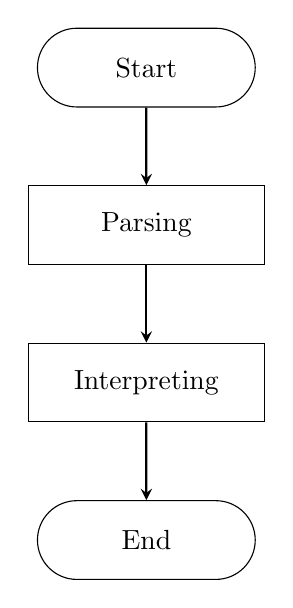
\begin{tikzpicture}[node distance=2cm]
		\node (start) [terminal] {Start};
		\node (parsing) [process, below of=start] {Parsing};
		\node (interpreting) [process, below of=parsing] {Interpreting};
		\node (end) [terminal, below of=interpreting] {End};
		\draw [flowchartarrow] (start) -- (parsing);
		\draw [flowchartarrow] (parsing) -- (interpreting);
		\draw [flowchartarrow] (interpreting) -- (end);
	\end{tikzpicture}
	\caption{The major steps carried out by an interpreter}
	\label{fig:interpreting_flowchart}
\end{figure}

The implementation language will be rust because it is a language the author is
familiar with and because it is a high performance language as it compiles to
machine code. This is very important when writing an interpreter because it
will allow to have acceptable performance. Writing an interpreter in an
interpreted language would accumulate overhead and result in bad performance.

\subsection{Parsing}

When parsing, the source code which can be gathered from various sources is
converted into an abstract syntax tree (AST) and then the AST is interpreted.

At first we were hoping to use tree-sitter as our parsing system because it
would give us syntax highlighting inside of editors without having to write a
regex based grammar or another parser. However writing tree-sitter grammars is
not an easy task and is described as having ``a difficult learning
curve''\cite{ts_creating_parsers}.

This is why we have decided to use a different method for parsing the code. We
settled on using parser combinators with the help of the parser combinator
framework \citetitle{nom}. This library was chosen because it is the most widely
used parsing framework for rust (our implementation language) and the author
has experience having used it while going through \textcite{eopl}.

Another advantage of using parser combinators is that they allow to perform
complex transformations during the parsing. For example, it is possible to
transform a switch statement into if statements and else-if statements into
if and else statements during the parsing instead of in a different pass, this
allows to reduce the complexity of subsequent passes at the cost of increasing
the complexity of the parser.

This advantage comes directly from another major advantage of using a parser
combinator based method: flexibility. The other major method would be to use a
parser generator library, the method recommended by \textcite{eopl}, such as
\textcite{bison}. The downside of this is that the program will have to be
built upon the structure of the parser and will be limited by it.

\subsubsection{Language Grammar}

The language grammar defines all the possible different statements and
expressions found in the language to simplify writing the parser. If we used a
method using parser generators we would normally have given our grammar to the
parser generator so it then generates the parser. In our case, because we are
writing the parser ourselves in order to be able to easily keep track of
everything that has to be implemented having a list of the statements,
expressions and other constructs allows us to easily keep track of everything.

\noindent
Statement ::= \texttt{global} Identifier \texttt{=} Expression\\
Statement ::= Identifier \texttt{=} Expression\\
Statement ::= \texttt{array} Identifier\texttt{[}\{Expression\}\textsuperscript{+(\texttt{,})}\texttt{]}\\
Statement ::= Expression\\
Statement ::= \texttt{for} Identifier \texttt{=} Expression \texttt{to} Expression List-of-Statements \texttt{next} Identifier\\
Statement ::= \texttt{while} Expression List-of-Statements \texttt{endwhile}\\
Statement ::= \texttt{do} List-of-Statements \texttt{until} Expression\\

\noindent
Statement ::= \texttt{if} Expression \texttt{then} List-of-Statements \{\texttt{elseif} Expression \texttt{then} List-of-Statements\}\textsuperscript{*} \{\texttt{else} List-of-Statements\}\textsuperscript{?} \texttt{endif}\\
Statement ::= \texttt{switch} Expression\texttt{:} \{\texttt{case} Expression\texttt{:} List-of-Statements\}\textsuperscript{*} \{\texttt{default:} List-of-Statements\}\textsuperscript{?} \texttt{endswitch}\\

\noindent
Statement ::= \texttt{function} Identifer\texttt{(}\{Identifier\{:byVal | :byRef\}\}\textsuperscript{*(\texttt{,})}\texttt{)} List-of-Statements \texttt{endfunction}\\
Statement ::= \texttt{procedure} Identifer\texttt{(}\{Identifier\{:byVal | :byRef\}\}\textsuperscript{*(\texttt{,})}\texttt{)} List-of-Statements \texttt{endprocedure}\\
Statement ::= \texttt{return} Expression\\

\noindent
List-of-Statements ::= ()\\
List-of-Statements ::= (Statement . List-of-Statements)\\

\noindent
Expression ::= Constant\\
Expression ::= Identifer\texttt{(}\{Expression\}\textsuperscript{*(\texttt{,})}\texttt{)}\\
Expression ::= Identifier\texttt{.}Field\\
Expression ::= Identifier\texttt{.}Method\texttt{(}\{Expression\}\textsuperscript{*(\texttt{,})}\texttt{)}\\

\noindent
Expression ::= Expression \texttt{AND} Expression\\
Expression ::= Expression \texttt{OR} Expression\\
Expression ::= \texttt{NOT} Expression\\

\noindent
Expression ::= Expression \texttt{==} Expression\\
Expression ::= Expression \texttt{!=} Expression\\
Expression ::= Expression \texttt{\textless{}} Expression\\
Expression ::= Expression \texttt{\textless=} Expression\\
Expression ::= Expression \texttt{\textgreater{}} Expression\\
Expression ::= Expression \texttt{\textgreater=} Expression\\

\noindent
Expression ::= Expression \texttt{+} Expression\\
Expression ::= Expression \texttt{-} Expression\\
Expression ::= Expression \texttt{*} Expression\\
Expression ::= Expression \texttt{/} Expression\\
Expression ::= Expression \texttt{MOD} Expression\\
Expression ::= Expression \texttt{DIV} Expression\\
Expression ::= Expression \texttt{\textasciicircum{}} Expression\\

\noindent
Program ::= List-of-Statements

The grammar is then used to write the parser including the structures that are
used:

\begin{minted}{rust}
#[derive(Debug, PartialEq, Clone)]
enum Expression<'a> {
    StringLiteral(&'a str),
    IntegerLiteral(i64),
    FloatLiteral(f64),
    BoolLiteral(bool),
    Identifier(&'a str),
    FunctionCall(&'a str, Vec<Expression<'a>>),
    Variable(&'a str),

    Equal(Box<Expression<'a>>, Box<Expression<'a>>),
    NotEqual(Box<Expression<'a>>, Box<Expression<'a>>),
    LessThan(Box<Expression<'a>>, Box<Expression<'a>>),
    LessThanOrEqual(Box<Expression<'a>>, Box<Expression<'a>>),
    GreaterThan(Box<Expression<'a>>, Box<Expression<'a>>),
    GreaterThanOrEqual(Box<Expression<'a>>, Box<Expression<'a>>),

    Plus(Box<Expression<'a>>, Box<Expression<'a>>),
    Minus(Box<Expression<'a>>, Box<Expression<'a>>),
    Times(Box<Expression<'a>>, Box<Expression<'a>>),
    Divide(Box<Expression<'a>>, Box<Expression<'a>>),
    Modulus(Box<Expression<'a>>, Box<Expression<'a>>),
    Quotient(Box<Expression<'a>>, Box<Expression<'a>>),
    Power(Box<Expression<'a>>, Box<Expression<'a>>),

    And(Box<Expression<'a>>, Box<Expression<'a>>),
    Or(Box<Expression<'a>>, Box<Expression<'a>>),
    Not(Box<Expression<'a>>),
}

#[derive(Debug, PartialEq)]
enum Statement<'a> {
    Assignment(&'a str, Expression<'a>),
    GlobalAssignment(&'a str, Expression<'a>),
    ArrayDefinition(&'a str, Vec<usize>),
    Expression(Expression<'a>),
    For(
        &'a str,
        Expression<'a>,
        Expression<'a>,
        ListOfStatements<'a>,
    ),
    While(Expression<'a>, ListOfStatements<'a>),
    If(Expression<'a>, ListOfStatements<'a>, ListOfStatements<'a>),
    // asRef: bool
    Function(&'a str, Vec<(&'a str, bool)>, ListOfStatements<'a>),
    Return(Expression<'a>),
}

type ListOfStatements<'a> = Vec<Statement<'a>>;
\end{minted}

\subsection{Interpreting}

\subsection{Testing}

In order to test the parser we are going to use the built-in unit testing
feature of Rust because they allow to simplify the process of testing with all
the already existing tools provided by rust, and is less error prone than
rolling out our own testing solution, using for example a custom script.

For example, we will be able to view our code coverage, a measure of how much
of the code is being tested by tests. Using this we will be able to add tests
to handle the under tested cases and have a measure of how much of the code is
tested and hence most likely to be correct.

By being able to quantitatively measure our testing strategy we can assure
ourself of the accuracy and reliability of our program.

\section{NOTES NOT PART OF REPORT}

Note on string literals: the unicode characters `“` and `”` seem to be used to
delimit string literals. Is that normal??

In the examples given, different unicode characters are used, that's a bit
wacky.

Escaping doesn't seem to exist either

We'll assume identifiers cannot start with numbers (see alter, maybe this can
be changed)

What do we consider whitespace? is a zero width space whitespace?

Do we want to implement closures?? (for language? for implementation? for parsing? for interpreting?)

What are valid identifiers? We'll follow C with: only: letters, digits and
underscore, but first character must be letter or underscore.

Test cases shouldn't be called '*.input' they can contain actual programs so
that doesn't make sense.

%We do not have operator precedence (help)

%Rust doesn't support backtracking in macros:
%https://github.com/rust-lang/rust/issues/24827, https://github.com/rust-lang/rust/issues/42838
so we had to inverse the direction of our ops macro

%Use pretty_assertions to speed up AST testing

Fuzz the parser (idk why, we should just do it cause that sounds cool)

Switch statement implemented as a bunch of if else

This language makes no sense. For example, switch statements have a colon after
the expression. WHY?

On (physical) page 39, there is a 1, after `case "B"`, wtf

Switch statement if given complex expression will compute expression at every
check

Log:

%Changed from ../ to CARGO_MANIFEST_DIR

alt((
	value(x, x),
	value(x, x),
	value(x, x),
	value(x, x),
))

was failing to compile. So I had to report it to the authors.

There is no "break" statement for loops.

Array is defined as "array" and "Array" in the spec...

Fields in classes must be defined before methods.

For loops will rewrite the counter variable, so the user can change it.
Pascal prevents compilation of programs where the variable is changed so I
think that's a fine behaviour.

For dealing with when to return a float or integer, we are following python's
behaviour. E.g. division always returns float (exception, thinking logically
seems to have issues with the new code) (update: so I asked Mrs Zeshan to show
me the solution to the homework to be 100\% of the correct. Turns out what I
had was correct. So the issue is with the interpreter or PG Online having
terrible questions/mark schemes.

Power return integer or other depending on various things

Problem, test with stdout
Solution: allow to write to other places than stdout

Problem: numerical values can be ints or floats.
Solution: fail no silently whenever types are somewhat not similar and
comparing the 2 hasn't explicitly been defined.

This behaviour is different than what python does. Python will happily compare
an integer and a string, always returning False.

Another way in which the behaviour is away from python is that when we print a
float, if it doesn't have any decimal place it shows like an int. This is
because we use the rust formatter. Although we have said we try to emulate
python behaviour, we will probably use rust behaviour before.

Programmed wasm support in browser it works!!!! I'm a bit wary of performance
issues with stuff being copied.

Fixed performance issue potentially (idk didn't benchmark) but we still have
the problem that the dom won't redraw in this infinite loop...

Tried using xterm js, reached a problem where the input was corrupted. This was
solved by using .slice(): https://github.com/rustwasm/wasm-bindgen/issues/1668

The problem is that even with xterm js the output doesn't show.

Last solution: using a background worker.

Couldn't load web worker. Turns out it's because Firefox doesn't support web
workers as modules.

The solution is to load it dynamically or smth now it works. It's weird how we
have to receive the message first before we can load the module.

Fixed a bug with integer literal parsing where "-1" would be detected a
variable

Could have used something like https://github.com/mitsuhiko/insta to improve
development speed.

Added a reference type which in the end I had to remove, nevermind, I'll just
extend it, why am I so retarded 😖

We need to implement returning from functions inside of execute\_statements

\subsection{Where to find example code}

\begin{itemize}
	\item In the specification
	\item Unit 10 Computational thinking, Homework 4 Thinking logically
\end{itemize}

\printbibliography[heading=bibintoc]

\end{document}
